\documentclass[letta4 paper]{article}
% Set target color model to RGB
\usepackage[inner=2.0cm,outer=2.0cm,top=2.5cm,bottom=2.5cm]{geometry}
\usepackage{setspace}
\usepackage[rgb]{xcolor}
\usepackage{verbatim}
\usepackage{subcaption}
\usepackage{amsgen,amsmath,amstext,amsbsy,amsopn,tikz,amssymb,tkz-linknodes}
\usepackage{fancyhdr}
\usepackage[colorlinks=true, urlcolor=blue,  linkcolor=blue, citecolor=blue]{hyperref}
\usepackage[colorinlistoftodos]{todonotes}
\usepackage{rotating}
\usepackage{listings}
\lstset{
%	language=bash,
	basicstyle=\ttfamily
}

\newcommand{\ra}[1]{\renewcommand{\arraystretch}{#1}}

\newtheorem{thm}{Theorem}[section]
\newtheorem{prop}[thm]{Proposition}
\newtheorem{lem}[thm]{Lemma}
\newtheorem{cor}[thm]{Corollary}
\newtheorem{defn}[thm]{Definition}
\newtheorem{rem}[thm]{Remark}
\numberwithin{equation}{section}
\graphicspath{ {./img/} }

\newcommand{\homework}[6]{
   \pagestyle{myheadings}
   \thispagestyle{plain}
   \newpage
   \setcounter{page}{1}
   \noindent
   \begin{center}
   \framebox{
      \vbox{\vspace{2mm}
    \hbox to 6.28in { {\bf F1TENTH Autonomous Racing \hfill {\small (#2)}} }
       \vspace{6mm}
       \hbox to 6.28in { {\Large \hfill #1  \hfill} }
       \vspace{6mm}
       \hbox to 6.28in { {\it Instructor: {\rm #3} \hfill Name: {\rm #5}, StudentID: {\rm #6}} }
       %\hbox to 6.28in { {\it T\textbf{A:} #4  \hfill #6}}
      \vspace{2mm}}
   }
   \end{center}
   \markboth{#5 -- #1}{#5 -- #1}
   \vspace*{4mm}
}


\newcommand{\problem}[3]{~\\\fbox{\textbf{Problem #1: #2}}\hfill (#3 points)\newline}
\newcommand{\subproblem}[1]{~\newline\textbf{(#1)}}
\newcommand{\D}{\mathcal{D}}
\newcommand{\Hy}{\mathcal{H}}
\newcommand{\VS}{\textrm{VS}}
\newcommand{\solution}{~\newline\textbf{\textit{(Solution)}} }

\newcommand{\bbF}{\mathbb{F}}
\newcommand{\bbX}{\mathbb{X}}
\newcommand{\bI}{\mathbf{I}}
\newcommand{\bX}{\mathbf{X}}
\newcommand{\bY}{\mathbf{Y}}
\newcommand{\bepsilon}{\boldsymbol{\epsilon}}
\newcommand{\balpha}{\boldsymbol{\alpha}}
\newcommand{\bbeta}{\boldsymbol{\beta}}
\newcommand{\0}{\mathbf{0}}


\usepackage{booktabs}



\begin{document}

	\homework {Lab 2: Automatic Emergency Braking}{Due Date:}{INSTRUCTOR}{}{STUDENT NAME}{ID}
	\thispagestyle{empty}
		
	\begin{table}[h]
		\begin{tabular}{l p{14cm}}
		\raisebox{-2cm}{
\includegraphics[scale=0.5, height=2.5cm]{f1_stickers_04} } & \textit{This lab and all related course material on \href{http://f1tenth.org/}{F1TENTH Autonomous Racing} has been developed by the Safe Autonomous Systems Lab at the University of Pennsylvania (Dr. Rahul Mangharam). It is licensed under a \href{https://creativecommons.org/licenses/by-nc-sa/4.0/}{Creative Commons Attribution-NonCommercial-ShareAlike 4.0 International License.} You may download, use, and modify the material, but must give attribution appropriately. Best practices can be found \href{https://wiki.creativecommons.org/wiki/best_practices_for_attribution}{here}.}
		\end{tabular}
	\end{table}
	
	
	\noindent \large{\textbf{Course Policy:}} Read all the instructions below carefully before you start working on the assignment, and before you make a submission. All sources of material must be cited. The University Academic Code of Conduct will be strictly enforced.
	
	\section{Learning outcomes}

	The following fundamentals should be understood by the students upon completion of this lab:
		
	\begin{itemize}
		\item Using the LaserScan message in ROS
		\item Time to Collision (TTC)
		\item Safety critical systems
	\end{itemize}
	
	\section{Overview}
	The goal of this lab is to develop a safety node for the race cars that will stop the car from collision when travelling at higher velocities. We will implement Time to Collision (TTC) using the \texttt{LaserScan} message in the simulator. 
	
	\subsection{The \texttt{LaserScan} Message}
	
	Recall from the previous lab that each LaserScan message contains several fields that will be useful to us. You’ll need to subscribe to the scan topic and calculate TTC with the \texttt{LaserScan} messages.
	
	\subsection{The \texttt{Odometry} Message}
	
	Both the simulator node and the car itself publish Odometry messages (ROS documentation linked here: \url{http://docs.ros.org/melodic/api/nav msgs/html/msg/Odometry.html}). Within its several fields, the message in- cludes the car’s position, orientation, and velocity. You’ll need to explore this message type in this lab.
	
	\subsection{The \texttt{AckermannDriveStamped} Message}
	
	\texttt{AckermannDriveStamped} is the message type that we’ll use throughout the course to send driving commands to the simulator and the car. ROS’s documentation is linked here:
	\url{http://docs.ros.org/api/ackermann msgs/html/msg/AckermannDriveStamped.html}
	Note that we won’t be sending driving commands to the car from this node, we’re only sending the brake commands. By sending an \texttt{AckermannDriveStamped} message with the velocity set to 0.0, the simulator and the car will interpret this as a brake command and hit the brakes.
	
	\subsection{The TTC Calculation}
	
	Time to Collision (TTC) is the time it would take for the car to collide with an obstacle if it maintained its current heading and velocity. Between the car and its obstacle, we can calculate it as:
	
	\[
	TTC = \frac{r}{[-\dot{r}]_+} 
	\]	
	
	where \(r\) is the distance between the two objects and \(\dot{r}\) is the time derivative of that distance. \(\dot{r}\) is computed by projecting the relative velocity of the car onto the distance vector between the two objects. The operator \([ ]_+\) is defined as: \([x]_+ := max(x,0)\).
	
	You'll need to calculate the TTC for each beam in the laser scan. Projecting the velocity of the car onto each distance vector is very simple if you know the angle between the car’s velocity vector and the distance vector (which can be determined easily from information in the \texttt{LaserScan} message).
	
	\section{Automatic Emergency Braking with TTC}
	
	For this lab, you will make a Safety Node that should halt the car before it collides with obstacles. To do this, you will make a ROS node that subscribes to the \texttt{LaserScan} and \texttt{Odometry} messages. It should analyze the \texttt{LaserScan} data and, if necessary, publish an \texttt{AckermannDriveStamped} with the velocity field set to 0.0 m/s, and a \texttt{Bool} message set to True (\url{http://docs.ros.org/melodic/api/std msgs/html/msg/Bool.html}). The \texttt{AckermannDriveStamped} message will be received by the \texttt{Mux} node and the \texttt{Bool} message will be received by the Behavior Controller, which will then tell the \texttt{Mux} node to select the appropriate \texttt{Drive} message.
	
	Note the following topic names for your publishers and subscribers (also detailed in the skeleton code): 
	
	\begin{itemize}
		\item LaserScan: “/scan”
		\item Odometry: “/odom”
		\item Bool message: “/brake bool”
		\item Brake message: “/brake”
	\end{itemize}
	
	You can implement this node in either C++ or Python, the skeleton code for both is found in the \texttt{f1tenth/f110\_ros} repository in the safety folder: \url{https://github.com/f1tenth/f110_ros}.
	\\
	\\
	\textbf{NOTE:} Make sure to press \textbf{’B’} on your keyboard in the terminal window that launched the simulator. This will activate the AEB and allow the Behavior Controller to switch the Mux to Emergency Brake when the boolean is published as True. Pressing \textbf{’B’} again will toggle the AEB off.
	
	\section{Deliverables and Submission}
	
	Submit the following as \texttt{studentname\_lab2.zip} (replace studentname with your name):
	

	\begin{enumerate}
		\item Your package including the safety node, named as \texttt{studentname\_safety}. \textbf{Make sure it compiles before you submit after changing the package name.}
		\item Make a youtube video of teleop (manual driving) around the Levine loop (with your safety node on) in the simulator without significant false positives. Add this link to a text file named \texttt{studentname\_lab2\_video.txt}
	\end{enumerate}

	\section{Grading}
	
	We will test your code by accelerating the car down a straight towards a wall in the Levine map, and your safety node should stop the car before collision.
	
	\subsection{Rubric}
	\begin{table}[h]
		\begin{tabular}{ll}
			\textbf{Topics} & \textbf{Points} \\
			Compilation & 30 \\
			Provided Video & 20 \\
			Correctly stops before collision & 30 \\
			Correctly calculates TTC & 10 \\
			Able to navigate through the hallway & 10 \\
			\textbf{Total} & 100 \\
		\end{tabular}
	\end{table}
	
	\newpage
	\section{FAQ}
		
	\textbf{Q:} How should the TTC threshold be determined? \\
	\textbf{A:} We recommend trial and error on a variety of situations (e.g. driving down the hall vs straight at a wall) to minimize false positives while preventing crashes. You can get a good initial estimate using the car’s deceleration (8.26 \(\frac{m}{s^2}\) ) and it’s velocity for keyboard driving (1.8 m \(\frac{m}{s}\))
	\\
	\\
	\textbf{Q:} Should “false” be published on the \texttt{brake bool} topic when the AEB is not in effect?\\
	\textbf{A:} Yes. Publishing “false” will make sure that no Drive messages on the brake topic are sent to the Simulator, and will allow other controllers (e.g. keyboard) to take back control.
	\\
	\\
	\textbf{Q:} If the AEB is not engaged, should a \texttt{AckermannDriveStamped} message be published on the brake topic?\\
	\textbf{A:} No, the \texttt{brake} topic is meant to only have messages that bring the car to a stop, so there is no need to send anything in this case. Moreover, if the AEB is not engaged, messages on the brake topic will not be sent to the Simulator.
	\\
	\\
	\textbf{Q:} Does the order of messages published matter? That is, is there a difference between:\\ \texttt{brake\_publisher.publish(brake\_msg);}\\
	\texttt{brake\_bool\_publisher.publish(brake\_bool\_msg);}\\
	and\\
	\texttt{brake\_bool\_publisher.publish(brake\_bool\_msg);}\\
	\texttt{brake\_publisher.publish(brake\_msg);}\\
	\textbf{A:} No. Due to latency between sending and receiving messages, this realistically won’t matter.
	\\
	\\
	\textbf{Q:} How are the coordinate frames of the \texttt{LaserScan} and \texttt{Odometry} data oriented with respect to the car?\\
	\textbf{A:} The \texttt{Odometry} data is in the frame centered on the rear axle, seen below. The message gives the magnitude and sign of the car’s velocity. It is always directed in the \texttt{+x} direction (red axis). The \texttt{LaserScan} data is in the LiDar’s frame, seen below towards the front of the car.
	\begin{center}
		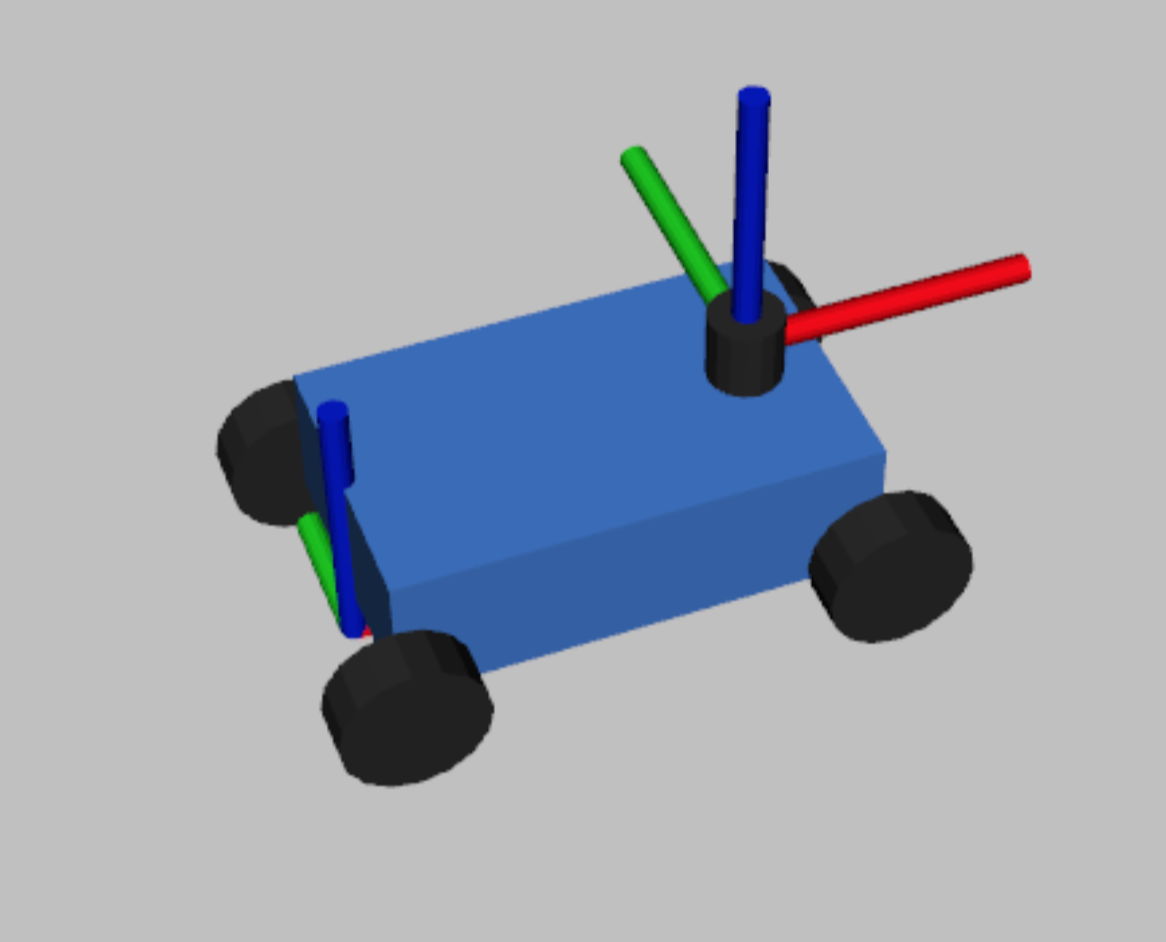
\includegraphics[scale=0.25]{car.png}
	\end{center}
	
	\noindent \textbf{Q:} When testing driving forwards and in reverse, the car’s distance from the wall after braking seems different between these two cases. Am I doing something wrong, or should I try and use different TTC thresholds?\\
	\textbf{A:} The ranges in the \texttt{LaserScan} message are from the LiDar’s frame (seen above) which is not in the center of the car. An ideal AEB system would subtract the distance from the LiDar to the edge of the car for each beam, and use that distance in the TTC calculation. A two-threshold system could work too, but for this assignment, as long as it doesn’t crash during keyboard teleop, a single threshold value is good enough. More sophisticated solutions are always welcome!
	\\
	\\
	\textbf{Q:} After the car is stopped by the AEB, if I drive the car towards the wall again, it will be stopped by the brake again. But if I repeat this, the car will move closer and closer to the wall until a collision occurs before the AEB can stop the car. Is this be acceptable or should the AEB prevent collisions in all circumstances?\\
	\textbf{A:} A collision in this unique situation is fine. When the car is extremely close to the wall and begins to move, it is impossible to stop it in time.	
		
		
			
\end{document} 
